\section{Aufbau des Magnetpendels}
\label{sec:aufbau_des_magnetpendels}

\paragraph{Realität} Ein Magnetpendel ist ein Versuchsaufbau aus der Physik, der oft zur Verdeutlichung von chaotischen Systemen bzw. schwacher Kausalität verwendet wird \comp{cornilsen1993magnetpendel}. Hauptkomponente ist der Pendelmagnet, ein Magnet, der an einer Stange unter seinem Ankerpunkt hängt und frei schwingen kann. In geringem Abstand unter dem Pendelmagneten befindet sich der Boden des Versuchsaufbaus, auf dem einige Magnete fixiert sind. Diese sind im Bezug auf deren Polung so befestigt, dass jeder den Pendelmagneten anzieht. Ihre Anordnung folgt dabei meist einem bestimmten Muster. In der Regel werden sie in gleichmäßigem Abstand um den Mittelpunkt des Bodens angeordnet. Bei einer geraden Anzahl dieser Fixmagnete ergibt sich also eine zum Mittelpunkt des Bodens punktsymmetrische Anordnung. Die zwischen den Fixmagneten und dem Pendelmagneten auftretende resultierende Anziehungskraft muss so groß sein, dass sie den Pendelmagnet entgegen der Schwerkraft außerhalb seiner Ruheposition festhalten kann. Wird der Pendelmagnet ausgelenkt, so wird er während des Pendelvorgangs ständig von den Fixmagneten abgelenkt, bis er schließlich so viel Energie verloren hat, dass er die Anziehung eines einzelnen Magneten nicht mehr überwinden kann und er über diesem zum Stehen kommt. Dabei kann die Endposition aufgrund der Einflussnahme durch die Fixmagnete schon durch minimale Änderung der Startposition komplett verändert werden.

\begin{figure}
    \includegraphics{aufbau}
	\caption{Skizze des Magnetpendels}
    \label{fig:skizze_des_magnetpendels}
\end{figure}

\paragraph{Modell} Das Modell stellt ein solches Magnetpendel dreidimensional dar. Wie in Abbildung \ref{fig:skizze_des_magnetpendels} zu sehen ist, liegt der Ursprung $0$ des Koordinatensystems auf dem Ankerpunkt des Pendelmagneten $P$. Die Länge der Verbindungsstange zwischen $0$ und $P$ beträgt $1m$. Die beiden fixierten Magnete $A$ und $B$ sind auf dem theoretischen Boden des Modells, der Ebene $E: -1,05m = z$, platziert. Ausgehend vom Mittelpunkt des Bodens $M(0m|0m|-1,05m)$ ist der Fixmagnet $A$ um $5cm$ in negative y-Richtung und der Fixmagnet $B$ um den selben Betrag in positive y-Richtung verschoben.

Das Modell weicht in zwei Punkten von seinem realen Vorbild ab. Zunächst sind die Magnete als elektrostatische Kugeln implementiert, sodass sie eine elektrische Ladung aufweisen. Dies ist der Tatsache geschuldet, dass magnetische Anziehungskräfte sehr schwer zu berechnen sind, da Magnete Dipole sind und ein sehr unregelmäßiges Magnetfeld ausbilden, wenn sie sich gegenseitig beeinflussen. Die Anziehungskräfte zwischen geladenen Kugeln hingegen lassen sich mit den Regeln der Elektrostatik exakt und effizient berechnen. Im Zusammenhang damit ist zu beachten, dass, auch wenn es sich im Modell um elektrisch geladene Kugeln handelt, diese zugunsten des Sprachflusses weiterhin als Magnete bezeichnet werden können. Die zweite Abweichung vom realen Vorbild besteht darin, dass die Verbindungsstange des Pendelmagneten keine Dicke aufweist. Sie wird somit bei der Berechnung des Strömungswiderstandes vernachlässigt.

Jeder Magnet ist somit durch seine Ladung $Q$ und seine Position $\vec{p}$ definiert. Der bewegliche Pendelmagnet besitzt zusätzlich eine Geschwindigkeit $\vec{v}$, eine Beschleunigung $\vec{a}$, eine auf ihn wirkende, resultierende Kraft $\vec{F}_{res}$ sowie eine Masse $m$ und einen Radius $r$.

